\documentclass{article}
\usepackage[title]{appendix}
\usepackage{authblk}
\usepackage{mathptmx}
\usepackage{url,latexsym,amsmath,amsthm,xspace,rotating,multirow,multicol,xspace,amssymb,paralist}
\usepackage{euscript}
\usepackage{fancybox,xcolor}
\usepackage{longtable}
\usepackage{paralist}
\usepackage[normalem]{ulem}
\usepackage[pdftex]{hyperref}
\usepackage{algorithmicx}
\usepackage{algpseudocode}
\usepackage{algorithm}
\usepackage{cancel}
\usepackage{mathtools}

\usepackage{url}
\usepackage{latexsym}

\usepackage{times}
\usepackage{amsmath}
\usepackage{amsthm}
\usepackage{amssymb}
\usepackage{graphicx}
\usepackage{xspace}
\usepackage{tabularx}
\usepackage{multicol}
\usepackage{multirow}
%\usepackage{hyperref}
\usepackage{url}
%\usepackage{natbib}
\usepackage{wrapfig}
\usepackage{comment}
\usepackage{listings}
\usepackage{color}
\usepackage[utf8]{inputenc}
\usepackage{fancyvrb}
\usepackage{booktabs}
\usepackage{color}
\usepackage[normalem]{ulem}

\usepackage{textcomp}

\newcommand{\obs}{\text{obs}}
\newcommand{\mis}{\text{mis}}

\newcommand{\qt}[1]{\left<#1\right>}
\newcommand{\ql}[1]{\left[#1\right]}
\newcommand{\hess}{\mathbf{H}}
\newcommand{\jacob}{\mathbf{J}}
\newcommand{\hl}{HL}
\newcommand{\cost}{\mathcal{L}}
\newcommand{\lout}{\mathbf{r}}
\newcommand{\louti}{r}
\newcommand{\outi}{y}
\newcommand{\out}{\mathbf{y}}
\newcommand{\gauss}{\mathbf{G_N}}
\newcommand{\eye}{\mathbf{I}}
\newcommand{\softmax}{\text{softmax}}
\newcommand{\targ}{\mathbf{t}}
\newcommand{\metric}{\mathbf{G}}
\newcommand{\sample}{\mathbf{z}}
\newcommand{\f}{\text{f}}
%\newcommand{\log}{\text{log}}

\newcommand{\bmx}[0]{\begin{bmatrix}}
\newcommand{\emx}[0]{\end{bmatrix}}
\newcommand{\qexp}[1]{\left<#1\right>}
\newcommand{\vect}[1]{\mathbf{#1}}
\newcommand{\vects}[1]{\boldsymbol{#1}}
\newcommand{\matr}[1]{\mathbf{#1}}
\newcommand{\var}[0]{\operatorname{Var}}
\newcommand{\std}[0]{\operatorname{std}}
\newcommand{\cov}[0]{\operatorname{Cov}}
\newcommand{\diag}[0]{\operatorname{diag}}
\newcommand{\matrs}[1]{\boldsymbol{#1}}
\newcommand{\va}[0]{\vect{a}}
\newcommand{\vb}[0]{\vect{b}}
\newcommand{\vc}[0]{\vect{c}}
\newcommand{\ve}[0]{\vect{e}}

\newcommand{\vh}[0]{\vect{h}}
\newcommand{\vv}[0]{\vect{v}}
\newcommand{\vx}[0]{\vect{x}}
\newcommand{\vp}[0]{\vect{p}}
\newcommand{\vz}[0]{\vect{z}}
\newcommand{\vw}[0]{\vect{w}}
\newcommand{\vs}[0]{\vect{s}}
\newcommand{\vf}[0]{\vect{f}}
\newcommand{\vi}[0]{\vect{i}}
\newcommand{\vo}[0]{\vect{o}}
\newcommand{\vd}[0]{\vect{d}}
\newcommand{\vy}[0]{\vect{y}}
\newcommand{\vg}[0]{\vect{g}}
\newcommand{\vm}[0]{\vect{m}}
\newcommand{\vu}[0]{\vect{u}}
\newcommand{\vL}[0]{\vect{L}}
\newcommand{\vr}[0]{\vect{r}}
\newcommand{\vone}[0]{\vect{1}}

\newcommand{\mW}[0]{\matr{W}}
\newcommand{\mE}[0]{\matr{E}}
\newcommand{\mG}[0]{\matr{G}}
\newcommand{\mX}[0]{\matr{X}}
\newcommand{\mY}[0]{\matr{Y}}
\newcommand{\mQ}[0]{\matr{Q}}
\newcommand{\mB}[0]{\matr{B}}
\newcommand{\mU}[0]{\matr{U}}
\newcommand{\mF}[0]{\matr{F}}
\newcommand{\mV}[0]{\matr{V}}
\newcommand{\mA}{\matr{A}}
\newcommand{\mC}{\matr{C}}
\newcommand{\mD}{\matr{D}}
\newcommand{\mL}[0]{\matr{L}}
\newcommand{\mR}[0]{\matr{R}}
\newcommand{\mS}{\matr{S}}
\newcommand{\mI}{\matr{I}}
\newcommand{\td}[0]{\text{d}}
\newcommand{\TT}[0]{\vects{\theta}}
\newcommand{\vsig}[0]{\vects{\sigma}}
\newcommand{\valpha}[0]{\vects{\alpha}}
\newcommand{\vmu}[0]{\vects{\mu}}
\newcommand{\vzero}[0]{\vect{0}}
\newcommand{\tf}[0]{\text{m}}
\newcommand{\tdf}[0]{\text{dm}}
\newcommand{\grad}[0]{\nabla}
\newcommand{\alert}[1]{\textcolor{red}{#1}}
\newcommand{\N}[0]{\mathcal{N}}
\newcommand{\YY}[0]{\mathcal{Y}}
\newcommand{\BB}[0]{\mathcal{B}}
\newcommand{\LL}[0]{\mathcal{L}}
\newcommand{\HH}[0]{\mathcal{H}}
\newcommand{\RR}[0]{\mathbb{R}}
\newcommand{\MM}[0]{\mathcal{M}}
\newcommand{\OO}[0]{\mathbb{O}}
\newcommand{\II}[0]{\mathbb{I}}
\newcommand{\Scal}[0]{\mathcal{S}}
\newcommand{\sigmoid}{\sigma}
\newcommand{\sign}{\text{sign}}
\newcommand{\E}[0]{\mathbb{E}}
\newcommand{\enabla}[0]{\ensuremath{%
    \overset{\raisebox{-0.3ex}[0.5ex][0ex]{%
    \ensuremath{\scriptscriptstyle e}}}{\nabla}}}
\newcommand{\enhnabla}[0]{\nabla_{\hspace{-0.5mm}e}\,}
\newcommand{\eos}[0]{\ensuremath{\left< \text{eos}\right>}}


\newcommand{\todo}[1]{{\Large\textcolor{red}{#1}}}
\newcommand{\done}[1]{{\Large\textcolor{green}{#1}}}
\newcommand{\dd}[1]{\ensuremath{\mbox{d}#1}}

\DeclareMathOperator*{\argmax}{\arg \max}
\DeclareMathOperator*{\argmin}{\arg \min}
\newcommand{\newln}{\\&\quad\quad{}}

\newcommand{\BP}{\text{BP}}
\newcommand{\PPL}{\text{PPL}}
\newcommand{\PL}{\text{PL}}
\newcommand{\MatSum}{\text{MatSum}}
\newcommand{\MatMul}{\text{MatMul}}
\newcommand{\KL}{\text{KL}}
\newcommand{\data}{\text{data}}
\newcommand{\rect}{\text{rect}}
\newcommand{\maxout}{\text{maxout}}
\newcommand{\train}{\text{train}}
\newcommand{\hinge}{\text{hinge}}
\newcommand{\val}{\text{val}}
\newcommand{\init}{\text{init}}
\newcommand{\fenc}{\text{fenc}}
\newcommand{\renc}{\text{renc}}
\newcommand{\enc}{\text{enc}}
\newcommand{\dec}{\text{dec}}
\newcommand{\test}{\text{test}}
\newcommand{\tra}{\text{tra}}
\newcommand{\Ax}{\mathcal{A}_x}
\newcommand{\Ay}{\mathcal{A}_y}
\newcommand{\ola}{\overleftarrow}
\newcommand{\ora}{\overrightarrow}
\newcommand{\ov}{\overline}
\newcommand{\ts}{\rule{0pt}{2.6ex}}       % Top strut
\newcommand{\ms}{\rule{0pt}{0ex}}         % Middle strut
\newcommand{\bs}{\rule[-1.2ex]{0pt}{0pt}} % Bottom strut
\newcommand{\specialcell}[2][c]{%
  \begin{tabular}[#1]{@{}c@{}}#2\end{tabular}}


%\usepackage{bibentry}
%\nobibliography*

\begin{document}
\title{Methods for Projecting Population Growth}
\author{Ross Freeman}
\date{\today}
\maketitle
\section{Introduction}

Population growth is one of the many models of great importance to the scientific community. These models are used to predict the challenges and changes needed in the near and longterm future as the world's population inevitably grows. It is such an important subject that the UN frequently discusses new and better ways of modelling the future population. This has led to a number of competing models, each with its own strengths and weaknesses. While no model can be perfect, some have come relatively close to matching existing data and predict reasonable growth in the future. 

In order to understand just a how a few of these models operate, this paper will explore 3 separate models: standard logistic growth (LG), logistic growth augmented with migration data (LGM), and a modified Lotka-Volterra model (MLV). Each model has its own strengths and weaknesses and perform differently in comparison to actual data provided by the United Nations World Bank.

\section{Logistic Growth}

The Logistic Growth model is colloquially defined as:

\begin{align}
\label{eq:log-growth}
	P(t) = \frac{K N_0 e^{\gamma t}}{K + N_0 (e^{\gamma t} - 1)}
\end{align}
with $K$ being the theoretical maximum sustainable population, $N_0$ the initial population at time $t_0$, $\gamma$ being the yearly growth rate, and $t$ being the time since $t_0$.

While $N_0$ is trivially obtained from the dataset, $\gamma$ and $K$ are not so simple to obtain. These values are optimized utilizing the least squares method on the dataset, which contains census data since 1910. This produces a model that very closely matches the data, as seen in Figure 1.

\begin{figure}[ht!]
\centering
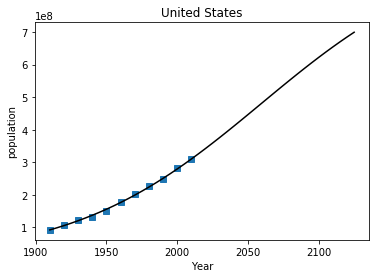
\includegraphics[width=90mm]{images/lr-graph.png}
\caption{Results of using least squares on logistic growth \label{overflow}}
\end{figure}

\todo{Finish details}

\section{Augmented Logistic Growth}

\todo{Fill in details}

\section{Modified Lotka-Volterra}

One theorized way to model population growth is in terms of economic growth of the human population, which can be seen as being equivalent to GDP. As GDP grows, the human population naturally grows with it due to an increase in the amount of output produced by the whole population. An interesting way to model this dynamic is through a modified version of the classic Lotka-Volterra model, which simulates the interaction between predators and prey. The population can be seen as the predator with GDP as the prey since the human population is theorized to grow with GDP up to a certain point, where it slightly decreases and reaches an equilibrium. However, there are numerous theories as to how GDP and population should be viewed together, so it is more appropriate to view the model in a more general sense. 

\subsection{Transforming Lotka-Volterra}

As discussed earlier in this course, the Lotka-Volterra model in it's most basic form is written as:

\begin{align}
\begin{split}
\label{eq:lv1}
	\frac{dp}{dt} = ap - rpg \\
	\frac{dg}{dt} = rpg - bg
\end{split}
\end{align}
where $p$ is the population of the prey, $g$ is the population of the predators, and $\frac{dp}{dt}$ and $\frac{dg}{dt}$ are their annual population changes. $rpg$ describes the interaction between the two species with $r$ being a regulating coefficient, $a$ being the growth rate of the prey in the absence of predators, and $b$ being the death rate of the predators in the absence of prey. Assuming $g$ and $p$ have the same variation, then the ratio $\frac{g}{p}$ can be evaluated to a constant ${q}$. \ref{eq:lv1} can then be rewritten as:

\begin{align}
\begin{split}
\label{eq:lv2}
	\frac{dp}{dt} = ap - rqp^2\\
	\frac{dg}{dt} = \frac{r}{q}g^2- bg
\end{split}
\end{align}

In order to account for other causes of variation that are not in the predator-prey system, the model can once again be modified to include a function $f(p, g, t)$. This can be seen as a function that modulates the growth of the prey in relation to a theoretical maximum capacity (i.e. due to the lack of natural resources). \ref{eq:lv2} can now be rewritten as:

\begin{align}
\begin{split}
\label{eq:lv3}
	\frac{dp}{dt} = (\alpha_1 + \alpha_3 f)p + \alpha_2 g p \\
	\frac{dg}{dt} = \beta_1 g + \beta_2 p g
\end{split}
\end{align}
where $a, b, r$ have been replaced by $\alpha_1, \alpha_2, \beta_1, \beta_2$, which now also contain the signs. $\alpha_3f$ modulates the growth rate $\alpha_1$

From here, the model can finally be adapted to the population growth problem. $p$ can be defined as the population and $g$ as the GDP at time $t$. Putting the model into context, the function $f$ can now be determined to finally derive an appropriate model from this problem.

The most logical choice for $f$ should be an equation that reflects changing technology that improves the human population's lifestyle. This is often cited by economists as being related to GDP per capita, or $\frac{g}{p}$. $f$ can then be set as $k_1 \frac{g}{p}$ where $k_1$ is some constant that regulates the effects of GDP per capita. Using that in equation \ref{eq:lv3} yields:

\begin{align}
\begin{split}
\label{eq:lvfin}
	\frac{dp}{dt} = \alpha_1 p + \alpha_3 k_1 g + \alpha_2 g p \\
	\frac{dg}{dt} = \beta_1 g + \beta_2 p g
\end{split}
\end{align}

It is appropriate to now put the coefficients into context for a better understanding of how the model functions. $\alpha_1$ is the growth rate of the population in the absence of other factors, in terms of percentage. Similarly, $\beta_1$ is the growth rate of GDP in the absence of other factors. $\alpha_2$ and $\beta_2$ describe the interaction between population and GDP and should be negative. $\alpha_2$ is in terms of $\frac{1}{US\$}$ and $\beta_2$ is in terms of $\frac{1}{Hab.}$. $\alpha_3 k_1$ describes the positive affect that GDP has on the human population and is in terms of $\frac{Hab.}{US\$}$. In other words, it describes how many more people are born for each additional dollar that is added to the GDP. 

\subsection{Initial Simulation}

The model's authors derived what they found to be appropriate values for the parameters above when adapting the model to a global scale. The values used are: $T_0 = 1850$, $T_f = 2100$, step size $D_T = 1.0$, $P_0 = 1.15$ billion inhabitants, $G_0 = 0.21$ trillion US\$, $\alpha_1 = 0.3\%$, $\alpha_2 = \frac{-55}{10^{18} US\$}$, $\alpha_3 k_1 = 5.2 \frac{Hab.}{US \$}$, $\beta_1 = 3.1\%$, and $\beta_2 = \frac{-2}{10^{22} Hab.}$. 

As the authors note, the model follows a logistic growth curve initially, as is expected for initial population growth. At a certain point though, the population actually begins to decrease, a significant divergence from the logistic growth model. This can be seen as a result of slowing technological growth and families becoming smaller as they become more financially stable. The population eventually levels out at an equilibrium just below 10 billion people. Meanwhile, GDP steadily grows at a sustained rate of about 1.5\%. GDP per capita is constantly rising throughout this period as technology also continues to improve. The authors point out, however, that a number of factors can have significant impacts on this model. In particular, major economic crises or significant technological achievement can raise or lower the equilibrium population. 

\subsection{Additional Simulation}

\todo{Complete Jupyter simulations}

\subsection{Analysis}

\todo{Analyze results}

\newpage

\begin{appendices}
\section{Simulation Code}
\todo{Insert actual code with comments}

\begin{lstlisting}[language=Python]
def model(params):   
    a1, a3k1, a2, b1, b2 = params
    # Sample comment
    def dpdt(x, t):
        return (a1*x[0] + a3k1*x[1] + a2*x[0]*x[1])
    def dgdt(x, t):
        return b1*x[1] + b2*x[0]*x[1]
    def dxdt(x, t):
        return np.array([dpdt(x, t),  dgdt(x, t)])
    
    x0 = [1.15e9, 0.21e12]
    t = np.arange(1850, 2150, 1)
    return integrate.odeint(dxdt, x0, t)
\end{lstlisting}

\end{appendices}

\newpage

\nocite{*}
\bibliographystyle{abbrv}
\bibliography{paper}

\end{document}